\documentclass[tikz,border=5pt]{standalone}
\usepackage{ctex}
\usepackage{amsmath}
\usetikzlibrary{arrows.meta,calc,angles,quotes}

\begin{document}
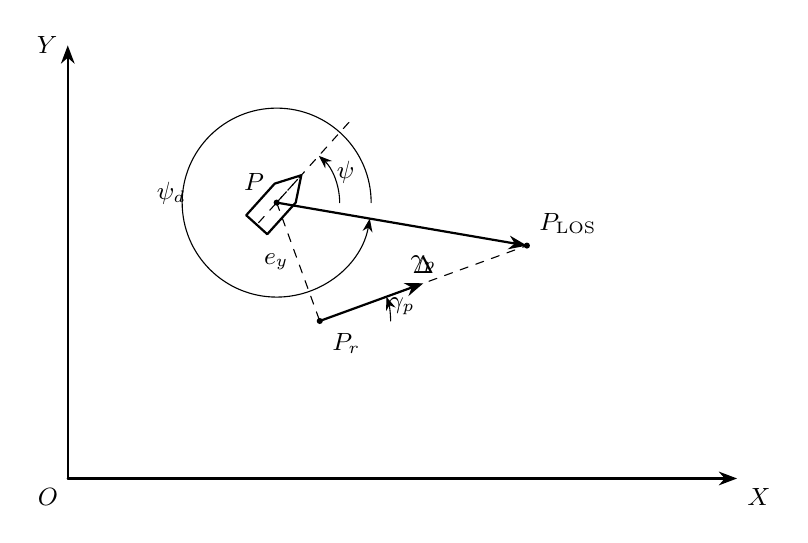
\begin{tikzpicture}[
    >=Stealth,
    line join=round,
    line cap=round,
    font=\small
]

% ======================================
% 参数设置
% ======================================
\def\gammaPath{20}      % 路径切向角 gamma_p
\def\lookahead{2.8}     % 前视距离 Delta
\def\ey{1.6}            % 横向误差 e_y
\def\psiCur{48}         % 当前航向 psi

% ======================================
% 全局坐标系
% ======================================
\coordinate (O) at (0,0);
\draw[->, thick] (O) -- (8.5,0) node[below right] {$X$};
\draw[->, thick] (O) -- (0,5.5) node[left] {$Y$};
\node[below left] at (O) {$O$};

% ======================================
% 参考路径：取一直线
% 路径上的投影点 Pr
% ======================================
\coordinate (Pr) at (3.2,2.0);

% 路径方向单位向量和法向方向
\coordinate (Tdir) at ({cos(\gammaPath)},{sin(\gammaPath)});
\coordinate (Ndir) at ({-sin(\gammaPath)},{cos(\gammaPath)});

% % 参考路径线段
% \draw[thick] ($(Pr)+(-4.2*cos(\gammaPath),-4.2*sin(\gammaPath))$)
%           -- ($(Pr)+(4.8*cos(\gammaPath),4.8*sin(\gammaPath))$)
%           node[above right] {Reference path};

% 路径切向短箭头
\draw[->, thick] (Pr) -- ++({1.4*cos(\gammaPath)},{1.4*sin(\gammaPath)})
    node[above] {$\gamma_p$};

% ======================================
% 当前USV位置 P
% P = Pr + e_y * normal
% ======================================
\coordinate (P) at ($(Pr)+({\ey*(-sin(\gammaPath))},{\ey*(cos(\gammaPath))})$);

\fill (Pr) circle (1.1pt);
\node[below right=1pt] at (Pr) {$P_r$};

\fill (P) circle (1.1pt);
\node[above left=1pt] at (P) {$P$};

% 横向误差线
\draw[dashed] (P) -- (Pr);
\node[left] at ($(P)!0.5!(Pr)$) {$e_y$};

% ======================================
% LOS前视点 P_LOS
% ======================================
\coordinate (PLOS) at ($(Pr)+({\lookahead*cos(\gammaPath)},{\lookahead*sin(\gammaPath)})$);

\fill (PLOS) circle (1.1pt);
\node[above right=1pt] at (PLOS) {$P_{\mathrm{LOS}}$};

% 前视距离 Delta
\draw[dashed] (Pr) -- (PLOS);
\node[above] at ($(Pr)!0.5!(PLOS)$) {$\Delta$};

% 期望航向连线
\draw[->, thick] (P) -- (PLOS);

% ======================================
% 当前USV俯视简图
% ======================================
\begin{scope}[shift={(P)}, rotate=\psiCur]
    \def\L{0.9}
    \def\W{0.36}
    \draw[thick]
        (-0.42*\L,-0.5*\W)
        -- (0.18*\L,-0.5*\W)
        -- (0.52*\L,0)
        -- (0.18*\L,0.5*\W)
        -- (-0.42*\L,0.5*\W)
        -- cycle;
    \draw[dashed] (-0.38*\L,0) -- (0.46*\L,0);
\end{scope}

% ======================================
% 当前航向 psi 的方向辅助线
% ======================================
\coordinate (PsiEnd) at ($(P)+({1.4*cos(\psiCur)},{1.4*sin(\psiCur)})$);
\draw[dashed] (P) -- (PsiEnd);

% 期望航向 psi_d 的方向点
% 从 P 指向 PLOS
\path let
    \p1 = ($(PLOS)-(P)$)
in
    coordinate (PsiDEnd) at ($(P)+( {1.55*(\x1)/veclen(\x1,\y1)} , {1.55*(\y1)/veclen(\x1,\y1)} )$);

% ======================================
% 画角度：gamma_p, psi, psi_d
% ======================================

% gamma_p: 从 X 轴到路径切向
\coordinate (XrefPr) at ($(Pr)+(1.3,0)$);
\draw pic[
    draw,
    ->,
    angle radius=9mm,
    angle eccentricity=1.18,
    "$\gamma_p$"
] {angle = XrefPr--Pr--PLOS};

% psi: 从 X 轴到当前航向
\coordinate (XrefP) at ($(P)+(1.2,0)$);
\draw pic[
    draw,
    ->,
    angle radius=8mm,
    angle eccentricity=1.2,
    "$\psi$"
] {angle = XrefP--P--PsiEnd};

% psi_d: 从 X 轴到期望航向
\draw pic[
    draw,
    ->,
    angle radius=12mm,
    angle eccentricity=1.12,
    "$\psi_d$"
] {angle = XrefP--P--PLOS};

\end{tikzpicture}
\end{document}